\newpage
\section{Estructuras}

\subsection{Segment Tree}
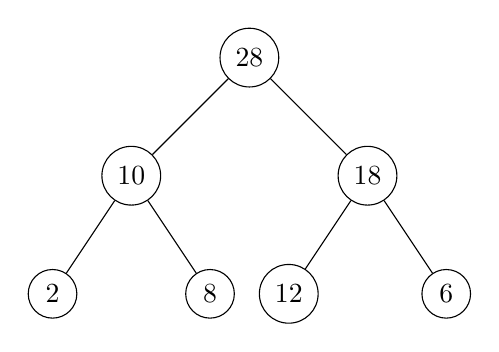
\begin{tikzpicture}[main/.style = {draw, circle}]
    % Nivel 1
    \node[main] (1) at (0,0) {28};

    % Nivel 2
    \node[main] (2) at (-1.5,-1.5) {10};
    \node[main] (3) at (1.5,-1.5) {18};

    % Nivel 3
    \node[main] (4) at (-2.5,-3) {2};
    \node[main] (5) at (-0.5,-3) {8};
    \node[main] (6) at (0.5,-3) {12};
    \node[main] (7) at (2.5,-3) {6};

    % Conexiones
    \draw (1) -- (2);
    \draw (1) -- (3);
    \draw (2) -- (4);
    \draw (2) -- (5);
    \draw (3) -- (6);
    \draw (3) -- (7);
\end{tikzpicture}

\lstinputlisting[language=C++]{secciones/estructuras/segment-tree.cpp}
\subsection{Array}
\lstinputlisting[language=C++]{secciones/estructuras/array.cpp}
\newpage
